\subsection{Валидация \texttt{nudisxs}}

Для проверки корректности расчётов полный спектр сечений, полученных с помощью \texttt{nudisxs}, был сопоставлен с экспериментальными данными по глубоконеупругому рассеянию нейтрино и антинейтрино на нуклонах. 
На рис.~\ref{fig:disxs_compare} показано сравнение предсказаний, полученных с помощью \texttt{XsDis}~\cite{kuzmin2006_finetuning,kuzmin2005_sumcc,kuzmin2006_axialmass} (на основе которых построен пакет \texttt{nudisxs}), с данными различных экспериментов, охватывающих диапазон энергий от единиц ГэВ до~$10^6$~ГэВ.

Наблюдается хорошее согласие с экспериментальными данными.

\begin{figure}[!h]
\centering
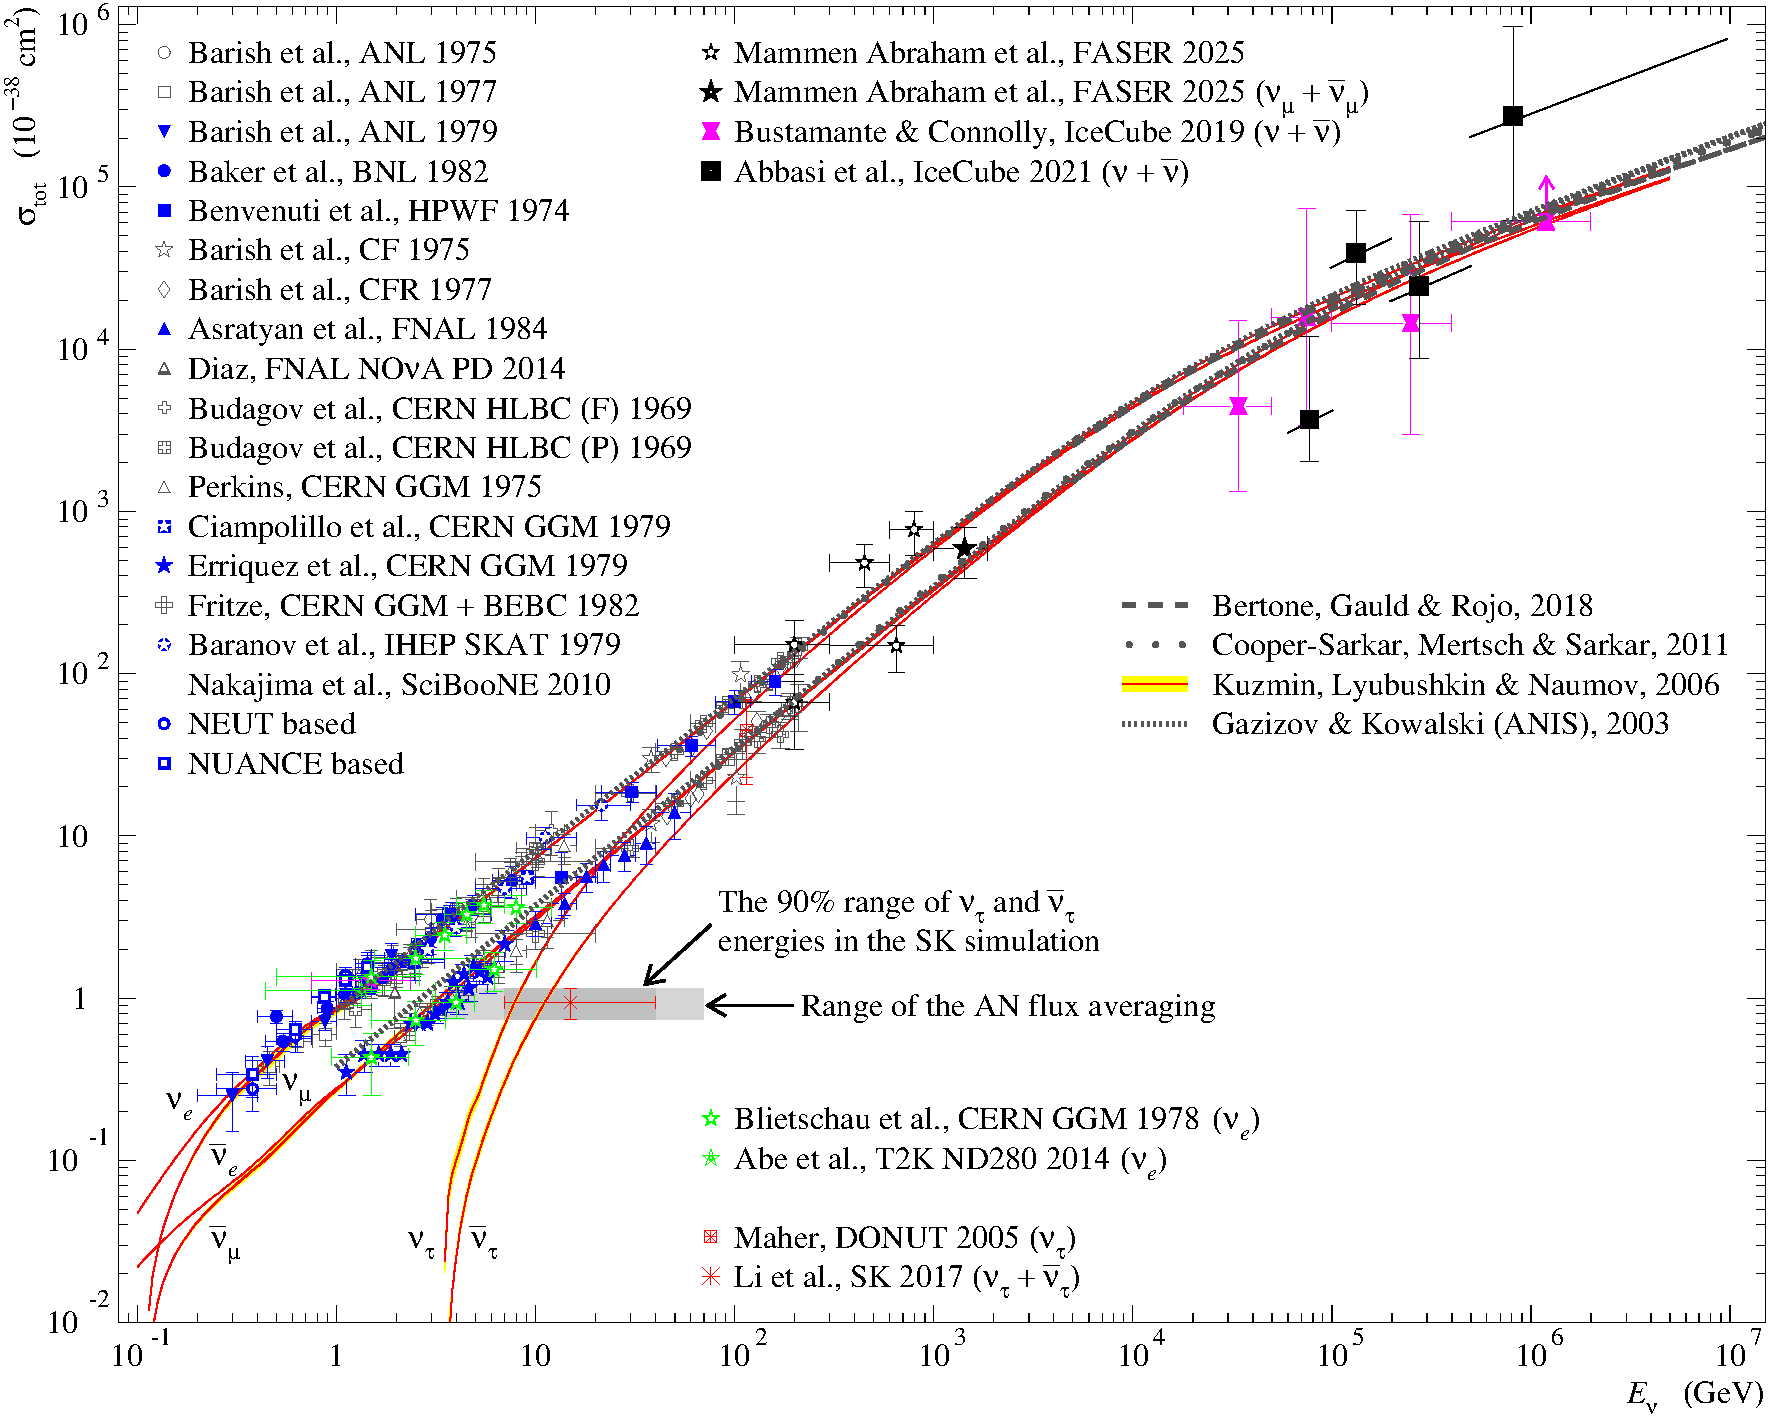
\includegraphics[width=\linewidth]{images/dis_vs_data.pdf}
\caption{Сравнение полного сечения глубоконеупругого рассеяния нейтрино и антинейтрино, рассчитанного с помощью \texttt{nudisxs}, с экспериментальными данными и теоретическими моделями~\cite{kuzmin2006_finetuning,kuzmin2005_sumcc,kuzmin2006_axialmass}.}
\label{fig:disxs_compare}
\end{figure}

